% ============================================================
%  J2 — MATIN : Classification Binaire & Perceptron
%  Julien Rolland — M2 Développement Fullstack
% ============================================================
\documentclass[aspectratio=169, 10pt]{beamer}
% ============================================================
%  PREAMBLE COMMUN — IA, Deep Learning & Machine Learning
%  Julien Rolland — M2 Développement Fullstack
% ============================================================

% --- Langue & encodage ---
\usepackage[utf8]{inputenc}
\usepackage[T1]{fontenc}
\usepackage{babel}
\babelprovide[import, main]{french}

% --- Thème Beamer ---
\usetheme{Madrid}
\usecolortheme{default}

% Palette de bleu académique
\definecolor{jedy_blue}{RGB}{0, 51, 102}       % bleu foncé principal
\definecolor{jedy_mid}{RGB}{0, 102, 179}        % bleu moyen accent
\definecolor{jedy_light}{RGB}{204, 221, 240}    % bleu très clair (fond boxes)
\definecolor{jedy_alert}{RGB}{180, 30, 30}      % rouge pour alertes
\definecolor{jedy_example}{RGB}{0, 120, 60}     % vert pour exemples

% Application des couleurs sur le thème Madrid
\setbeamercolor{palette primary}{bg=jedy_blue, fg=white}
\setbeamercolor{palette secondary}{bg=jedy_mid, fg=white}
\setbeamercolor{palette tertiary}{bg=jedy_blue, fg=white}
\setbeamercolor{palette quaternary}{bg=jedy_blue, fg=white}
\setbeamercolor{structure}{fg=jedy_blue}
\setbeamercolor{frametitle}{bg=jedy_blue, fg=white}
\setbeamercolor{title}{bg=jedy_blue, fg=white}
\setbeamercolor{block title}{bg=jedy_mid, fg=white}
\setbeamercolor{block body}{bg=jedy_light, fg=black}
\setbeamercolor{block title alerted}{bg=jedy_alert, fg=white}
\setbeamercolor{block body alerted}{bg=jedy_light, fg=black}
\setbeamercolor{block title example}{bg=jedy_example, fg=white}
\setbeamercolor{block body example}{bg=jedy_light, fg=black}

% --- Typographie ---
\usepackage{lmodern}
\setbeamerfont{title}{size=\Large, series=\bfseries}
\setbeamerfont{frametitle}{size=\normalsize, series=\bfseries}

% --- Navigation : suppression des icônes de navigation par défaut ---
\setbeamertemplate{navigation symbols}{}

% --- Numérotation des slides ---
\setbeamertemplate{footline}{%
  \leavevmode%
  \hbox{%
    \begin{beamercolorbox}[wd=.333\paperwidth,ht=2.25ex,dp=1ex,center]{author in head/foot}%
      \usebeamerfont{author in head/foot}\insertshortauthor
    \end{beamercolorbox}%
    \begin{beamercolorbox}[wd=.334\paperwidth,ht=2.25ex,dp=1ex,center]{title in head/foot}%
      \usebeamerfont{title in head/foot}\insertshorttitle
    \end{beamercolorbox}%
    \begin{beamercolorbox}[wd=.333\paperwidth,ht=2.25ex,dp=1ex,right]{date in head/foot}%
      \usebeamerfont{date in head/foot}
      \insertframenumber{} / \inserttotalframenumber\hspace*{2ex}
    \end{beamercolorbox}%
  }%
  \vskip0pt%
}

% --- Maths ---
\usepackage{amsmath, amssymb, amsthm}
\usepackage{bm}          % vecteurs en gras : \bm{w}

% --- Code source ---
\usepackage{listings}
\usepackage{xcolor}

\lstdefinestyle{pythonstyle}{
  language=Python,
  basicstyle=\ttfamily\footnotesize,
  keywordstyle=\color{jedy_blue}\bfseries,
  commentstyle=\color{gray}\itshape,
  stringstyle=\color{jedy_example},
  numberstyle=\tiny\color{gray},
  numbers=left,
  numbersep=5pt,
  frame=single,
  framerule=0.4pt,
  rulecolor=\color{jedy_light},
  backgroundcolor=\color{jedy_light!40},
  breaklines=true,
  showstringspaces=false,
  tabsize=4,
}
\lstset{style=pythonstyle}

% Alias pratique pour code inline
\newcommand{\code}[1]{\texttt{\small#1}}

% --- Graphiques ---
\usepackage{graphicx}
\usepackage{tikz}
\usetikzlibrary{arrows.meta, positioning, shapes.geometric, fit, calc}
\usepackage{pgfplots}
\pgfplotsset{compat=1.18}

% --- Tableaux ---
\usepackage{booktabs}
\usepackage{array}

% --- Icônes (optionnel, nécessite fontawesome5) ---
% \usepackage{fontawesome5}

% --- Macros ML/DL courantes ---
\newcommand{\R}{\mathbb{R}}
\newcommand{\E}{\mathbb{E}}
\newcommand{\Loss}{\mathcal{L}}
\newcommand{\dataset}{\mathcal{D}}
\newcommand{\X}{\mathbf{X}}
\newcommand{\y}{\mathbf{y}}
\newcommand{\w}{\mathbf{w}}
\newcommand{\W}{\mathbf{W}}
\newcommand{\grad}{\nabla}
\newcommand{\T}{^{\top}}         % transposée : \X\T
\newcommand{\lr}{\alpha}         % learning rate
\newcommand{\norm}[1]{\left\|#1\right\|}

% Encadré "Objectif pédagogique" en début de section
\newenvironment{objectif}{%
  \begin{alertblock}{Objectif}%
}{%
  \end{alertblock}%
}

% --- Infos du cours (remplacer dans chaque slides.tex) ---
\author[J. Rolland]{Julien Rolland}
\institute[Jedy]{Formation M2 Développement Fullstack}


\title[Classification \& Perceptron]{Classification Binaire \& Perceptron}
\subtitle{Jour 2 --- Matin}
\date{Jour 2}

% ============================================================
\begin{document}
% ============================================================

\begin{frame}
  \titlepage
\end{frame}

\begin{frame}{Plan du module}
  \tableofcontents
\end{frame}

% ============================================================
\section{Classification Binaire}
% ============================================================

\begin{frame}{De la Régression à la Classification}
  \begin{columns}[T]
    \begin{column}{0.50\textwidth}
      \textbf{Régression} (J1) : sortie \textbf{continue} $\hat{y}_i \in \R$

      \smallskip
      \textbf{Classification} (J2) : classe \textbf{discrète}
      $\hat{t}_n \in \{+1, -1\}$

      \smallskip
      \textbf{Exemples :}
      \begin{itemize}
        \item Email $\to$ spam / ham
        \item Image $\to$ chat / chien
        \item Tumeur $\to$ maligne / bénigne
      \end{itemize}

      \smallskip
      \begin{block}{Enjeu}
        Trouver une \textbf{frontière de décision} qui sépare
        les classes dans l'espace des features.
      \end{block}
    \end{column}
    \begin{column}{0.46\textwidth}
      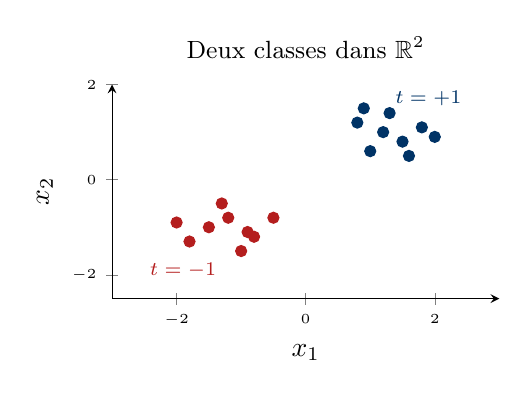
\begin{tikzpicture}
        \begin{axis}[
          width=6.5cm, height=4.3cm,
          xlabel={$x_1$}, ylabel={$x_2$},
          axis lines=left,
          tick label style={font=\tiny},
          xmin=-3, xmax=3, ymin=-2.5, ymax=2,
          title={\small Deux classes dans $\R^2$},
          title style={font=\small},
        ]
          \addplot[only marks, mark=*, mark size=2pt, jedy_blue]
            coordinates {
              (1.2,1.0)(1.5,0.8)(0.8,1.2)(1.8,1.1)(1.0,0.6)
              (1.3,1.4)(2.0,0.9)(1.6,0.5)(0.9,1.5)
            };
          \addplot[only marks, mark=*, mark size=2pt, jedy_alert]
            coordinates {
              (-1.5,-1.0)(-0.8,-1.2)(-1.2,-0.8)(-2.0,-0.9)(-1.0,-1.5)
              (-0.5,-0.8)(-1.8,-1.3)(-1.3,-0.5)(-0.9,-1.1)
            };
          \node[jedy_blue,  font=\scriptsize] at (axis cs: 1.9, 1.7) {$t=+1$};
          \node[jedy_alert, font=\scriptsize] at (axis cs:-1.9,-1.9) {$t=-1$};
        \end{axis}
      \end{tikzpicture}
    \end{column}
  \end{columns}
\end{frame}

% ---

\begin{frame}{Le Perceptron}
  \begin{columns}[T]
    \begin{column}{0.50\textwidth}
      \begin{block}{Modèle \& Prédiction}
        \[ f_\Theta(\bm{x}_n) = \w\T\bm{x}_n + b \in \R \]
        \[ \hat{t}_n = \operatorname{sign}(f_\Theta(\bm{x}_n))
           \in \{+1,-1\} \]
      \end{block}

      \smallskip
      Le signe de $f_\Theta(\bm{x}_n)$ indique de quel côté de
      l'hyperplan se trouve $\bm{x}_n$.
    \end{column}
    \begin{column}{0.46\textwidth}
      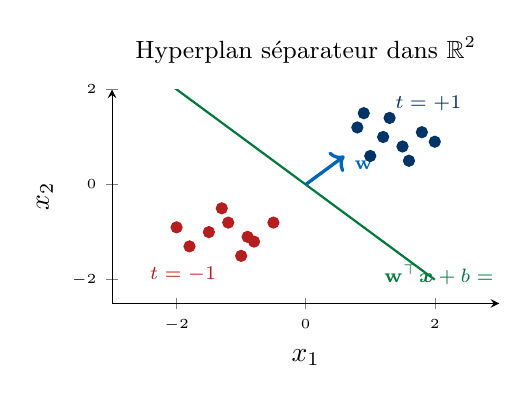
\begin{tikzpicture}
        \begin{axis}[
          width=6.5cm, height=4.3cm,
          xlabel={$x_1$}, ylabel={$x_2$},
          axis lines=left,
          tick label style={font=\tiny},
          xmin=-3, xmax=3, ymin=-2.5, ymax=2,
          title={\small Hyperplan séparateur dans $\R^2$},
          title style={font=\small},
        ]
          \addplot[only marks, mark=*, mark size=2pt, jedy_blue]
            coordinates {
              (1.2,1.0)(1.5,0.8)(0.8,1.2)(1.8,1.1)(1.0,0.6)
              (1.3,1.4)(2.0,0.9)(1.6,0.5)(0.9,1.5)
            };
          \addplot[only marks, mark=*, mark size=2pt, jedy_alert]
            coordinates {
              (-1.5,-1.0)(-0.8,-1.2)(-1.2,-0.8)(-2.0,-0.9)(-1.0,-1.5)
              (-0.5,-0.8)(-1.8,-1.3)(-1.3,-0.5)(-0.9,-1.1)
            };
          \addplot[jedy_example, thick, domain=-2.5:2.0] {-x};
          \draw[->, jedy_mid, very thick]
            (axis cs:0,0) -- (axis cs:0.6,0.6);
          \node[jedy_mid,     font=\scriptsize] at (axis cs: 0.9, 0.4) {$\w$};
          \node[jedy_example, font=\scriptsize] at (axis cs: 2.2,-1.9)
            {$\w\T\bm{x}+b=0$};
          \node[jedy_blue,    font=\scriptsize] at (axis cs: 1.9, 1.7) {$t=+1$};
          \node[jedy_alert,   font=\scriptsize] at (axis cs:-1.9,-1.9) {$t=-1$};
        \end{axis}
      \end{tikzpicture}
    \end{column}
  \end{columns}
\end{frame}

% ============================================================
\section{L'Impasse du Gradient}
% ============================================================

\begin{frame}{Pourquoi le Gradient Échoue}
  \begin{columns}[T]
    \begin{column}{0.50\textwidth}
      Pour optimiser $\Theta$ par descente de gradient :
      \[ \w \leftarrow \w - \lr\,\nabla_\w \Loss \]

      \smallskip
      \textbf{Problème :} le readout $\operatorname{sign}(z)$ est
      \textbf{non-différentiable} en $0$, dérivée \textbf{nulle} ailleurs.

      \smallskip
      \begin{alertblock}{Conséquences}
        \small
        \begin{itemize}
          \item $\operatorname{sign}$ dans la loss $\Rightarrow$
                $\nabla_\w \Loss = 0$ presque partout.
          \item Le gradient ne transporte \textbf{aucune information}.
          \item GD est \textbf{bloqué mathématiquement}.
        \end{itemize}
      \end{alertblock}

      \smallskip
      \begin{exampleblock}{Solution}
        Ne \textbf{pas} mettre le readout dans la loss.\\
        Utiliser une fonction \textbf{différentiable} à la place.
      \end{exampleblock}
    \end{column}
    \begin{column}{0.46\textwidth}
      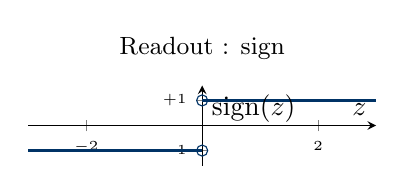
\begin{tikzpicture}
        \begin{axis}[
          width=6.0cm, height=2.6cm,
          xlabel={$z$}, ylabel={$\operatorname{sign}(z)$},
          axis lines=center,
          tick label style={font=\tiny},
          xmin=-3, xmax=3, ymin=-1.6, ymax=1.6,
          ytick={-1,1}, yticklabels={$-1$,$+1$},
          title={\small Readout : $\operatorname{sign}$},
          title style={font=\small},
        ]
          \addplot[jedy_blue, very thick, domain=-3:0] {-1};
          \addplot[jedy_blue, very thick, domain=0:3]  { 1};
          \addplot[only marks, mark=o, mark size=2pt, jedy_blue]
            coordinates {(0,-1)(0,1)};
        \end{axis}
      \end{tikzpicture}

      \smallskip
      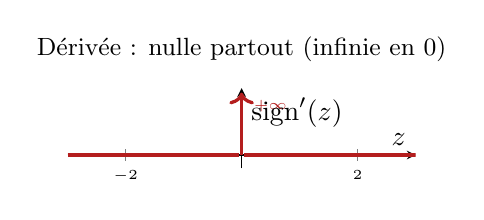
\begin{tikzpicture}
        \begin{axis}[
          width=6.0cm, height=2.6cm,
          xlabel={$z$}, ylabel={$\operatorname{sign}'(z)$},
          axis lines=center,
          tick label style={font=\tiny},
          xmin=-3, xmax=3, ymin=-0.3, ymax=1.5,
          ytick={0}, yticklabels={$0$},
          title={\small Dérivée : nulle partout (infinie en 0)},
          title style={font=\small},
        ]
          \addplot[jedy_alert, very thick, domain=-3:-0.05] {0};
          \addplot[jedy_alert, very thick, domain=0.05:3]   {0};
          \draw[->, jedy_alert, very thick]
            (axis cs:0,0) -- (axis cs:0,1.4);
          \node[jedy_alert, font=\tiny] at (axis cs:0.5,1.1) {$+\infty$};
        \end{axis}
      \end{tikzpicture}
    \end{column}
  \end{columns}
\end{frame}

% ============================================================
\section{ReLU \& Loss du Perceptron}
% ============================================================

\begin{frame}{ReLU --- La Fonction Clé}
  \begin{columns}[T]
    \begin{column}{0.50\textwidth}
      \begin{block}{Définition}
        \[ \operatorname{ReLU}(z) = \max(0,z) \]
      \end{block}

      \smallskip
      \begin{block}{Dérivée}
        \[
          \operatorname{ReLU}'(z) = \mathbf{1}[z > 0] =
          \begin{cases} 1 & z > 0 \\ 0 & z \leq 0 \end{cases}
        \]
      \end{block}

      \smallskip
      \textbf{Pourquoi c'est le standard :}
      \begin{itemize}
        \item Gradient \textbf{constant} ($= 1$) pour $z > 0$ ---
              l'information circule.
        \item Ultra-rapide : pas d'exponentielle.
        \item Atténue le \textit{Vanishing Gradient}
              (Deep Learning, J3).
      \end{itemize}
    \end{column}
    \begin{column}{0.46\textwidth}
      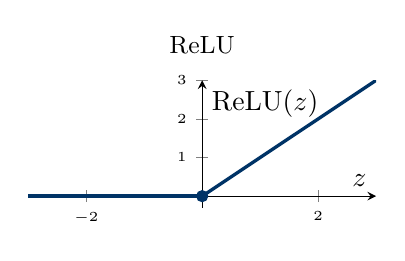
\begin{tikzpicture}
        \begin{axis}[
          width=6.0cm, height=3.2cm,
          xlabel={$z$}, ylabel={$\operatorname{ReLU}(z)$},
          axis lines=center,
          tick label style={font=\tiny},
          xmin=-3, xmax=3, ymin=-0.3, ymax=3,
          title={\small ReLU},
          title style={font=\small},
        ]
          \addplot[jedy_blue, very thick, domain=-3:0] {0};
          \addplot[jedy_blue, very thick, domain=0:3]  {x};
          \addplot[only marks, mark=*, mark size=2pt, jedy_blue]
            coordinates {(0,0)};
        \end{axis}
      \end{tikzpicture}

      \smallskip
      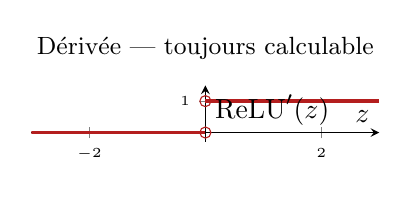
\begin{tikzpicture}
        \begin{axis}[
          width=6.0cm, height=2.3cm,
          xlabel={$z$}, ylabel={$\operatorname{ReLU}'(z)$},
          axis lines=center,
          tick label style={font=\tiny},
          xmin=-3, xmax=3, ymin=-0.3, ymax=1.5,
          ytick={0,1},
          title={\small Dérivée --- toujours calculable},
          title style={font=\small},
        ]
          \addplot[jedy_alert, very thick, domain=-3:0] {0};
          \addplot[jedy_alert, very thick, domain=0:3]  {1};
          \addplot[only marks, mark=o, mark size=2pt, jedy_alert]
            coordinates {(0,0)(0,1)};
        \end{axis}
      \end{tikzpicture}
    \end{column}
  \end{columns}
\end{frame}

% ---

\begin{frame}{Loss de Rosenblatt}
  \begin{columns}[T]
    \begin{column}{0.50\textwidth}
      \textbf{Idée :} mesurer l'erreur par le produit $f \cdot t_n$.
      \begin{itemize}
        \item $f \cdot t > 0$ : bonne classe $\Rightarrow$ perte $= 0$.
        \item $f \cdot t < 0$ : mauvaise classe $\Rightarrow$ pénalité.
      \end{itemize}

      \smallskip
      \begin{block}{Loss de Rosenblatt}
        \[
          \Loss = \frac{1}{N}\sum_{n=1}^{N}
          \operatorname{ReLU}\!\bigl(-f_\Theta(\bm{x}_n)\cdot t_n\bigr)
        \]
      \end{block}

      \smallskip
      Gradient pour un exemple \textbf{mal classifié}
      ($f \cdot t < 0$) :
      \[
        \nabla_\w \operatorname{ReLU}(-f\cdot t) = -t_n\,\bm{x}_n
      \]

      \begin{alertblock}{Règle de mise à jour}
        Si $\hat{t}_n \neq t_n$ :\quad
        $\w \leftarrow \w + \lr\, t_n\, \bm{x}_n$
      \end{alertblock}
    \end{column}
    \begin{column}{0.46\textwidth}
      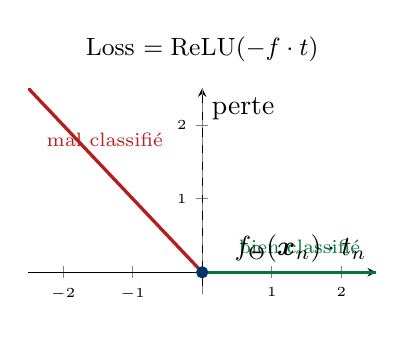
\begin{tikzpicture}
        \begin{axis}[
          width=6.0cm, height=4.2cm,
          xlabel={$f_\Theta(\bm{x}_n) \cdot t_n$},
          ylabel={perte},
          axis lines=center,
          tick label style={font=\tiny},
          xmin=-2.5, xmax=2.5, ymin=-0.3, ymax=2.5,
          title={\small Loss $= \operatorname{ReLU}(-f\cdot t)$},
          title style={font=\small},
          xtick={-2,-1,0,1,2},
        ]
          \addplot[jedy_example, very thick, domain=0:2.5]  {0};
          \addplot[jedy_alert,   very thick, domain=-2.5:0] {-x};
          \addplot[only marks, mark=*, mark size=2pt, jedy_blue]
            coordinates {(0,0)};
          \node[jedy_example, font=\scriptsize]
            at (axis cs: 1.4, 0.35) {bien classifié};
          \node[jedy_alert,   font=\scriptsize]
            at (axis cs:-1.4, 1.8) {mal classifié};
          \draw[dashed, gray, thin]
            (axis cs:0,-0.3) -- (axis cs:0,2.5);
        \end{axis}
      \end{tikzpicture}

      \smallskip
      \begin{exampleblock}{Encodage $\pm 1$ crucial}
        \small Avec $t \in \{0,1\}$, le produit $f \cdot t$
        serait nul pour la classe $0$ --- la loss
        ne fonctionnerait pas.
      \end{exampleblock}
    \end{column}
  \end{columns}
\end{frame}

% ============================================================
\section{Algorithme de Rosenblatt}
% ============================================================

\begin{frame}{Algorithme Online de Rosenblatt}
  \begin{columns}[T]
    \begin{column}{0.52\textwidth}
      \begin{block}{Algorithme}
        \small
        \textbf{Entrée :} $\bm{x}_1,\ldots,\bm{x}_N \in \R^D$,\;
        $t_1,\ldots,t_N \in \{+1,-1\}$,\; $\alpha$\\[4pt]
        $\tilde{\bm{x}}_n \leftarrow [1,\;\bm{x}_n\T]\T \in \R^{D+1}$
        \hfill\textit{(biais absorbé)}\\[2pt]
        $\bm{w} \leftarrow \vec{0} \in \R^{D+1}$\\[2pt]
        \textbf{pour} chaque époque \textbf{faire}\\
        \hspace{1.2em}\textbf{pour} $n = 1$ \textbf{à} $N$ \textbf{faire}\\
        \hspace{2.4em}$\hat{t}_n \leftarrow \operatorname{sign}(\bm{w}\T\tilde{\bm{x}}_n)$\\
        \hspace{2.4em}\textbf{si} $\hat{t}_n \neq t_n$ \textbf{alors}\\
        \hspace{3.6em}$\bm{w} \leftarrow \bm{w} + \alpha\, t_n\, \tilde{\bm{x}}_n$\\[2pt]
        \textbf{retourner} $\bm{w}$
      \end{block}

      \begin{alertblock}{« Online » = un exemple à la fois}
        \small Traite les données comme un \textbf{flux},
        pas comme un lot statique.
        Instable sur données \textbf{bruitées}.
      \end{alertblock}
    \end{column}
    \begin{column}{0.44\textwidth}
      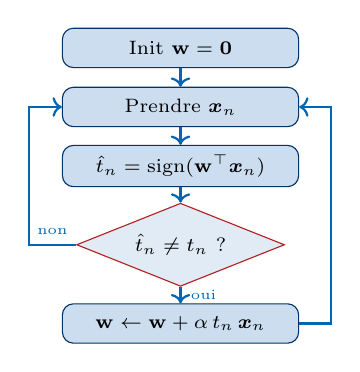
\begin{tikzpicture}[
        node distance=0.75cm,
        box/.style={draw=jedy_blue, fill=jedy_light, rounded corners,
                    minimum width=3.0cm, minimum height=0.5cm,
                    font=\scriptsize, align=center},
        dec/.style={draw=jedy_alert, fill=jedy_light!60,
                    diamond, aspect=2.5, minimum height=0.6cm,
                    font=\scriptsize, align=center},
        arr/.style={->, jedy_mid, thick},
      ]
        \node[box] (init)  {Init $\w = \bm{0}$};
        \node[box, below of=init]  (pick)
          {Prendre $\bm{x}_n$};
        \node[box, below of=pick]  (score)
          {$\hat{t}_n = \operatorname{sign}(\w\T\bm{x}_n)$};
        \node[dec, below of=score, node distance=1.0cm] (err)
          {$\hat{t}_n \neq t_n$ ?};
        \node[box, below of=err, node distance=1.0cm] (upd)
          {$\w \leftarrow \w + \lr\, t_n\, \bm{x}_n$};
        \draw[arr] (init)  -- (pick);
        \draw[arr] (pick)  -- (score);
        \draw[arr] (score) -- (err);
        \draw[arr] (err)   -- node[right, font=\tiny]{oui} (upd);
        \draw[arr] (upd.east)  -- ++(0.4,0) |- (pick.east);
        \draw[arr] (err.west)  --
          node[above, font=\tiny]{non} ++(-0.6,0) |- (pick.west);
      \end{tikzpicture}
    \end{column}
  \end{columns}
\end{frame}

% ---

\begin{frame}{Online vs Batch Gradient Descent}
  \begin{columns}[T]
    \begin{column}{0.55\textwidth}
      \small\begin{tabular}{lp{2.6cm}p{1.9cm}}
        \toprule
        \textbf{Stratégie} & \textbf{Gradient sur} & \textbf{Stabilité} \\
        \midrule
        Online (SGD pur) & 1 exemple & Très instable \\[0.3em]
        Mini-Batch       & $B$ exemples ($32$--$256$) & Bon équilibre \\[0.3em]
        Batch (full)     & Tout le dataset ($N$) & Très stable \\
        \bottomrule
      \end{tabular}

      \smallskip
      \begin{block}{Mini-Batch GD --- Pratique moderne}
        \small
        \begin{enumerate}
          \item Mélanger le dataset.
          \item Découper en batches de taille $B$.
          \item Pour chaque batch : gradient $\to$ update $\w$.
          \item Répéter sur toutes les \textbf{époques}.
        \end{enumerate}
      \end{block}
    \end{column}
    \begin{column}{0.41\textwidth}
      \begin{exampleblock}{Avantage clé : vectorisation}
        \small Un batch $(X_b, \bm{t}_b)$ de taille $B$ permet
        de calculer le gradient en un seul produit matriciel.\\
        Exploitable par \textbf{NumPy} et les \textbf{GPU}.
      \end{exampleblock}

      \smallskip
      \begin{alertblock}{Convergence}
        \small Si les données sont \textbf{linéairement séparables},
        le perceptron converge.\\
        Sinon : il oscille $\Rightarrow$ utiliser
        une loss différentiable.
      \end{alertblock}
    \end{column}
  \end{columns}
\end{frame}

% ============================================================
\section{Régression Logistique}
% ============================================================

\begin{frame}{Régression Logistique --- Sigmoïde \& Probabilités}
  \begin{columns}[T]
    \begin{column}{0.50\textwidth}
      Remplacer $\operatorname{sign}$ par une fonction \textbf{lisse}
      qui retourne une \textbf{probabilité}.

      \smallskip
      \begin{block}{Modèle \& Loss (BCE)}
        \small
        \[ \sigma(z) = \tfrac{1}{1+e^{-z}},\quad
           f_\Theta(\bm{x}_n) = \sigma(\w\T\bm{x}_n) \approx P(t_n{=}1 \mid \bm{x}_n) \]
        \[ \Loss_{\text{BCE}} = -\tfrac{1}{N}\sum_{n}
          \bigl[t_n \log f_n + (1-t_n)\log(1-f_n)\bigr] \]
      \end{block}

      \smallskip
      \begin{exampleblock}{Avantage}
        \small $\sigma$ diff.\ partout --- pénalise lourdement les erreurs confiantes ($\Loss\to+\infty$).
      \end{exampleblock}
    \end{column}
    \begin{column}{0.46\textwidth}
      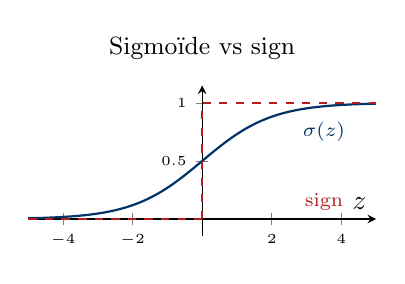
\begin{tikzpicture}
        \begin{axis}[
          width=6.0cm, height=3.5cm,
          xlabel={$z$},
          axis lines=center,
          tick label style={font=\tiny},
          xmin=-5, xmax=5, ymin=-0.15, ymax=1.15,
          ytick={0,0.5,1}, yticklabels={$0$,$0.5$,$1$},
          title={\small Sigmoïde vs $\operatorname{sign}$},
          title style={font=\small},
        ]
          \addplot[jedy_blue, thick, domain=-5:5, samples=100]
            {1/(1+exp(-x))};
          \addplot[jedy_alert, dashed, thick, domain=-5:-0.01] {0};
          \addplot[jedy_alert, dashed, thick, domain=0.01:5]   {1};
          \draw[jedy_alert, dashed, thick]
            (axis cs:0,0) -- (axis cs:0,1);
          \node[jedy_blue,  font=\scriptsize] at (axis cs:3.5,0.75) {$\sigma(z)$};
          \node[jedy_alert, font=\scriptsize] at (axis cs:3.5,0.15) {sign};
        \end{axis}
      \end{tikzpicture}
    \end{column}
  \end{columns}
\end{frame}

% ============================================================
\section{Architecture d'un Neurone}
% ============================================================

\begin{frame}{Un Neurone Artificiel}
  \begin{center}
    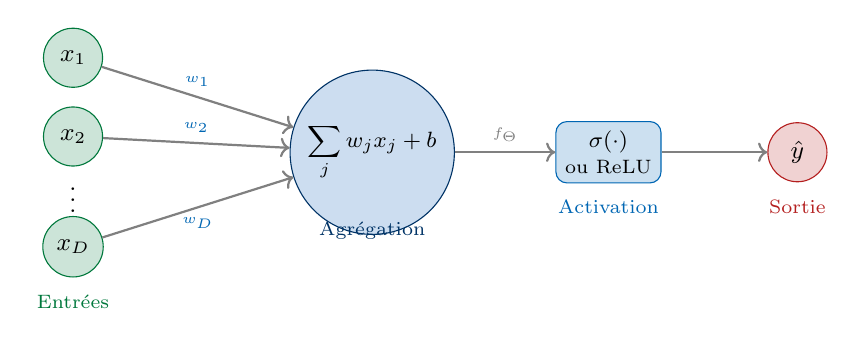
\begin{tikzpicture}[
      input/.style={circle, draw=jedy_example, fill=jedy_example!20,
                    minimum size=0.75cm, font=\small},
      neuron/.style={circle, draw=jedy_blue, fill=jedy_light,
                     minimum size=1.1cm, font=\footnotesize, align=center},
      activ/.style={rectangle, rounded corners, draw=jedy_mid,
                    fill=jedy_mid!20, minimum width=1.3cm,
                    minimum height=0.75cm, font=\footnotesize, align=center},
      outp/.style={circle, draw=jedy_alert, fill=jedy_alert!20,
                   minimum size=0.75cm, font=\small},
      arr/.style={->, thick, gray},
    ]
      \node[input]  (x1) at (0,  1.6) {$x_1$};
      \node[input]  (x2) at (0,  0.6) {$x_2$};
      \node[font=\small] at (0, -0.1) {$\vdots$};
      \node[input]  (xD) at (0, -0.8) {$x_D$};

      \node[neuron] (sum) at (3.8, 0.4)
            {$\displaystyle\sum_j w_j x_j + b$};

      \node[activ]  (act) at (6.8, 0.4)
            {$\sigma(\cdot)$\\\scriptsize ou ReLU};

      \node[outp]   (out) at (9.2, 0.4) {$\hat{y}$};

      \draw[arr] (x1) -- node[above, font=\tiny, jedy_mid]{$w_1$} (sum);
      \draw[arr] (x2) -- node[above, font=\tiny, jedy_mid]{$w_2$} (sum);
      \draw[arr] (xD) -- node[below, font=\tiny, jedy_mid]{$w_D$} (sum);
      \draw[arr] (sum) -- node[above, font=\tiny]{$f_\Theta$} (act);
      \draw[arr] (act) -- (out);

      \node[font=\scriptsize, jedy_example] at (0,   -1.5) {Entrées};
      \node[font=\scriptsize, jedy_blue]    at (3.8, -0.6) {Agrégation};
      \node[font=\scriptsize, jedy_mid]     at (6.8, -0.3) {Activation};
      \node[font=\scriptsize, jedy_alert]   at (9.2, -0.3) {Sortie};
    \end{tikzpicture}
  \end{center}

  \vspace{0.1cm}
  \begin{columns}[T]
    \begin{column}{0.48\textwidth}
      \begin{block}{Perceptron = réseau à 0 couche cachée}
        \small Entrées $\to$ agrégation $\to$ readout.\\
        Premier réseau de neurones (Rosenblatt, 1958).
      \end{block}
    \end{column}
    \begin{column}{0.48\textwidth}
      \begin{exampleblock}{Readout vs Activation}
        \small \textbf{Activation} : dans le réseau
        (ReLU, $\tanh$, $\sigma$) --- différentiable.\\
        \textbf{Readout} : décision finale
        ($\operatorname{sign}$, $\arg\max$).
      \end{exampleblock}
    \end{column}
  \end{columns}
\end{frame}

% ============================================================
\section{Classification Multi-Classes}
% ============================================================

\begin{frame}{Classification Multi-Classes}
  \begin{columns}[T]
    \begin{column}{0.50\textwidth}
      \textbf{Classification binaire} (jusqu'ici) :
      $\hat{t}_n \in \{+1,-1\}$

      \smallskip
      \textbf{Multi-classes} : $K$ catégories discrètes,
      $\hat{k} \in \{1, \ldots, K\}$

      \smallskip
      \textbf{Exemples :}
      \begin{itemize}
        \item Chiffres MNIST ($K = 10$)
        \item Objets CIFAR-10 ($K = 10$)
        \item Fleurs Iris ($K = 3$)
      \end{itemize}

      \smallskip
      \begin{block}{Enjeu}
        Séparer $K$ classes --- une \textbf{frontière de décision}
        par classe.
      \end{block}
    \end{column}
    \begin{column}{0.46\textwidth}
      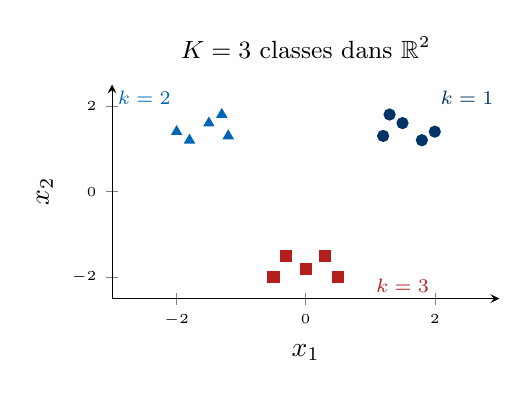
\begin{tikzpicture}
        \begin{axis}[
          width=6.5cm, height=4.3cm,
          xlabel={$x_1$}, ylabel={$x_2$},
          axis lines=left,
          tick label style={font=\tiny},
          xmin=-3, xmax=3, ymin=-2.5, ymax=2.5,
          title={\small $K = 3$ classes dans $\R^2$},
          title style={font=\small},
        ]
          \addplot[only marks, mark=*, mark size=2pt, jedy_blue]
            coordinates {(1.2,1.3)(1.5,1.6)(1.8,1.2)(1.3,1.8)(2.0,1.4)};
          \addplot[only marks, mark=triangle*, mark size=2pt, jedy_mid]
            coordinates {(-1.2,1.3)(-1.5,1.6)(-1.8,1.2)(-1.3,1.8)(-2.0,1.4)};
          \addplot[only marks, mark=square*, mark size=2pt, jedy_alert]
            coordinates {(-0.3,-1.5)(0.3,-1.5)(0,-1.8)(-0.5,-2.0)(0.5,-2.0)};
          \node[jedy_blue,  font=\scriptsize] at (axis cs: 2.5, 2.2) {$k=1$};
          \node[jedy_mid,   font=\scriptsize] at (axis cs:-2.5, 2.2) {$k=2$};
          \node[jedy_alert, font=\scriptsize] at (axis cs: 1.5,-2.2) {$k=3$};
        \end{axis}
      \end{tikzpicture}
    \end{column}
  \end{columns}
\end{frame}

% ---

\begin{frame}{Un Perceptron par Classe}
  \begin{columns}[T]
    \begin{column}{0.44\textwidth}
      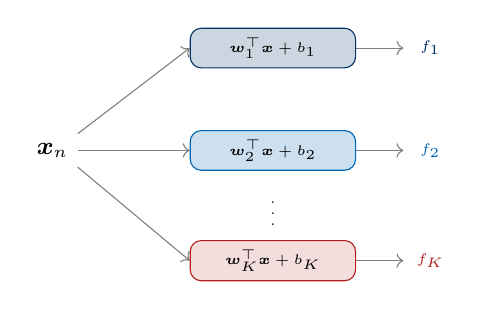
\begin{tikzpicture}[
        neur/.style={rectangle, rounded corners,
                     minimum width=2.1cm, minimum height=0.45cm,
                     font=\tiny, align=center, draw},
        arr/.style={->, gray, thin},
      ]
        \node[font=\small] (x) at (0, 1.5) {$\bm{x}_n$};

        \node[neur, draw=jedy_blue, fill=jedy_blue!20] (n1)
          at (2.8, 2.8) {$\bm{w}_1\T\bm{x}+b_1$};
        \node[neur, draw=jedy_mid, fill=jedy_mid!20] (n2)
          at (2.8, 1.5) {$\bm{w}_2\T\bm{x}+b_2$};
        \node[font=\tiny] at (2.8, 0.8) {$\vdots$};
        \node[neur, draw=jedy_alert, fill=jedy_alert!15] (nk)
          at (2.8, 0.1) {$\bm{w}_K\T\bm{x}+b_K$};

        \node[font=\tiny, jedy_blue]  at (4.8, 2.8) {$f_1$};
        \node[font=\tiny, jedy_mid]   at (4.8, 1.5) {$f_2$};
        \node[font=\tiny, jedy_alert] at (4.8, 0.1) {$f_K$};

        \draw[arr] (x.north east) -- (n1.west);
        \draw[arr] (x)            -- (n2.west);
        \draw[arr] (x.south east) -- (nk.west);

        \draw[arr] (n1.east) -- ++(0.6,0);
        \draw[arr] (n2.east) -- ++(0.6,0);
        \draw[arr] (nk.east) -- ++(0.6,0);
      \end{tikzpicture}

      \smallskip
      \small Score de la classe $k$ :
      \[ f_k(\bm{x}_n) = \bm{w}_k\T\bm{x}_n + b_k \in \R \]
    \end{column}
    \begin{column}{0.52\textwidth}
      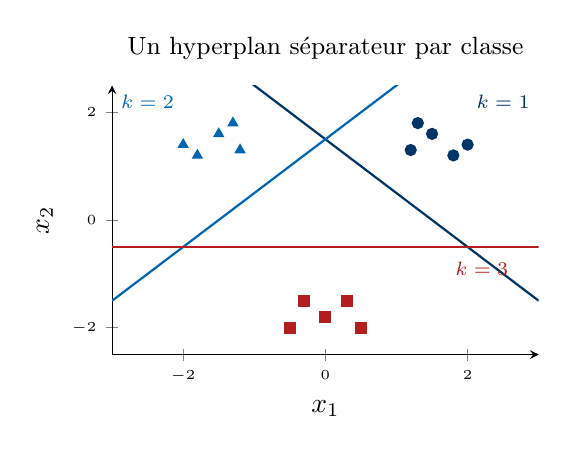
\begin{tikzpicture}
        \begin{axis}[
          width=7.0cm, height=5.0cm,
          xlabel={$x_1$}, ylabel={$x_2$},
          axis lines=left,
          tick label style={font=\tiny},
          xmin=-3, xmax=3, ymin=-2.5, ymax=2.5,
          title={\small Un hyperplan séparateur par classe},
          title style={font=\small},
        ]
          \addplot[only marks, mark=*, mark size=2pt, jedy_blue]
            coordinates {(1.2,1.3)(1.5,1.6)(1.8,1.2)(1.3,1.8)(2.0,1.4)};
          \addplot[only marks, mark=triangle*, mark size=2pt, jedy_mid]
            coordinates {(-1.2,1.3)(-1.5,1.6)(-1.8,1.2)(-1.3,1.8)(-2.0,1.4)};
          \addplot[only marks, mark=square*, mark size=2pt, jedy_alert]
            coordinates {(-0.3,-1.5)(0.3,-1.5)(0,-1.8)(-0.5,-2.0)(0.5,-2.0)};
          % Hyperplan k=1 : y = 1.5 - x  (sépare cluster 1 des deux autres)
          \addplot[jedy_blue,  thick, domain=-3:3] {1.5 - x};
          % Hyperplan k=2 : y = 1.5 + x  (sépare cluster 2 des deux autres)
          \addplot[jedy_mid,   thick, domain=-3:3] {1.5 + x};
          % Hyperplan k=3 : y = -0.5     (sépare cluster 3 des deux autres)
          \addplot[jedy_alert, thick, domain=-3:3] {-0.5};
          \node[jedy_blue,  font=\scriptsize] at (axis cs: 2.5, 2.2) {$k=1$};
          \node[jedy_mid,   font=\scriptsize] at (axis cs:-2.5, 2.2) {$k=2$};
          \node[jedy_alert, font=\scriptsize] at (axis cs: 2.2,-0.9) {$k=3$};
        \end{axis}
      \end{tikzpicture}
    \end{column}
  \end{columns}
\end{frame}

% ---

\begin{frame}{Softmax \& Prédiction}
  \begin{columns}[T]
    \begin{column}{0.52\textwidth}
      \begin{block}{Softmax $\to$ probabilités}
        \[
          p_k = \frac{e^{f_k}}{\displaystyle\sum_{j=1}^{K} e^{f_j}}
          \in (0,1), \qquad \sum_{k=1}^{K} p_k = 1
        \]
        \small Lisse et différentiable : adaptée à la descente de gradient.
      \end{block}

      \smallskip
      Les scores bruts $f_k$ (\textbf{logits}) sont convertis
      en distribution de probabilité sur les $K$ classes.
    \end{column}
    \begin{column}{0.44\textwidth}
      \begin{block}{Encodage \& Prédiction}
        \small $\bm{t}_n \in \{0,1\}^K$ (\textbf{one-hot}) :
        une seule composante à $1$.
        \[
          k=1 \;\to\; \begin{pmatrix}1\\0\\0\end{pmatrix}, \quad
          k=2 \;\to\; \begin{pmatrix}0\\1\\0\end{pmatrix}
        \]
        Readout : $\hat{k} = \arg\max_k\, p_k(\bm{x}_n)$
      \end{block}

      \smallskip
      \begin{exampleblock}{Exemple $K = 3$}
        \small
        \begin{tabular}{ll}
          Logits :     & $[3.0,\;1.5,\;0.5]$ \\[2pt]
          Softmax :    & $[0.77,\;0.17,\;0.06]$ \\[2pt]
          Prédiction : & $\hat{k} = 1$ \\
        \end{tabular}
      \end{exampleblock}
    \end{column}
  \end{columns}
\end{frame}

% ---

\begin{frame}{$K$ Perceptrons $=$ 1 Matrice}
  \begin{columns}[T]
    \begin{column}{0.52\textwidth}
      $K$ équations séparées, une par classe :
      \[
        f_k(\bm{x}_n) = \bm{w}_k\T\bm{x}_n + b_k,
        \quad k = 1, \ldots, K
      \]

      \begin{alertblock}{Empilement $\Rightarrow$ 1 équation matricielle}
        \[
          \underbrace{\bm{f}(\bm{x}_n)}_{\R^K}
          = \underbrace{\W}_{\R^{K\times D}}\,
            \underbrace{\bm{x}_n}_{\R^D}
          + \underbrace{\bm{b}}_{\R^K}
        \]
        \small Ligne $k$ de $\W$ = $\bm{w}_k\T$ (perceptron de classe $k$).
      \end{alertblock}

      \begin{block}{Forme batch (tout le dataset)}
        \small $\bm{F} = \bm{X}\W\T + \mathbf{1}_N\bm{b}\T$,
        \hfill $\bm{X}\in\R^{N\times D}$, $\bm{F}\in\R^{N\times K}$.\\
        1 seul produit matriciel pour les $N$ exemples.
      \end{block}
    \end{column}
    \begin{column}{0.44\textwidth}
      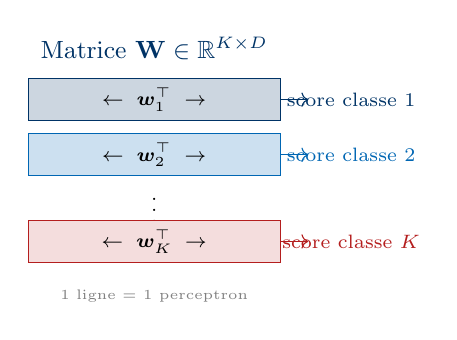
\begin{tikzpicture}[
        rbox/.style={rectangle, minimum width=3.2cm, minimum height=0.52cm,
                     font=\scriptsize, align=center, draw},
        arr/.style={->, thin},
      ]
        \node[font=\small, jedy_blue] at (0, 4.0)
          {Matrice $\W \in \R^{K\times D}$};

        \node[rbox, draw=jedy_blue, fill=jedy_blue!20] (r1) at (0, 3.35)
          {$\leftarrow\;\bm{w}_1\T\;\rightarrow$};
        \node[rbox, draw=jedy_mid, fill=jedy_mid!20] (r2) at (0, 2.65)
          {$\leftarrow\;\bm{w}_2\T\;\rightarrow$};
        \node[font=\scriptsize] at (0, 2.05) {$\vdots$};
        \node[rbox, draw=jedy_alert, fill=jedy_alert!15] (rk) at (0, 1.55)
          {$\leftarrow\;\bm{w}_K\T\;\rightarrow$};

        \node[jedy_blue,  font=\scriptsize] at (2.5, 3.35) {score classe $1$};
        \node[jedy_mid,   font=\scriptsize] at (2.5, 2.65) {score classe $2$};
        \node[jedy_alert, font=\scriptsize] at (2.5, 1.55) {score classe $K$};

        \draw[arr, jedy_blue]  (r1.east) -- ++(0.35,0);
        \draw[arr, jedy_mid]   (r2.east) -- ++(0.35,0);
        \draw[arr, jedy_alert] (rk.east) -- ++(0.35,0);

        \node[font=\tiny, gray, align=center] at (0, 0.85)
          {1 ligne = 1 perceptron};
      \end{tikzpicture}

      \smallskip
      \small
      $\bm{P} \in \R^{N\times K}$ : ligne $n$ = $\bm{p}_n$ (probas softmax de $\bm{x}_n$)\\
      $\bm{T} \in \R^{N\times K}$ : ligne $n$ = $\bm{t}_n$ (label one-hot de $\bm{x}_n$)
    \end{column}
  \end{columns}
\end{frame}

% ---

\begin{frame}{Loss CCE \& Gradients pour $\W$ et $\bm{b}$}
  \begin{columns}[T]
    \begin{column}{0.50\textwidth}
      \begin{block}{Cross-Entropy Catégorielle (CCE)}
        \[
          \Loss = -\frac{1}{N}\sum_{n}\sum_{k}
          t_{n,k}\,\log(p_{n,k})
        \]
        \small Seul le $\log$ de la \textbf{vraie classe} contribue
        ($t_{n,k}=0$ pour les autres).
      \end{block}

      \smallskip
      \begin{block}{Gradient w.r.t.\ les logits}
        \[
          \frac{\partial \Loss}{\partial f_{n,k}}
          = p_{n,k} - t_{n,k}
        \]
        \small Erreur $=$ proba prédite $-$ label one-hot.\\
        Résultat \textbf{élégant} : Softmax $+$ log $+$ CCE.
      \end{block}
    \end{column}
    \begin{column}{0.46\textwidth}
      \begin{block}{Gradients pour $\W$ et $\bm{b}$}
        \small Par règle de chaîne ($f_{n,k} = \bm{w}_k\T\bm{x}_n + b_k$) :
        \[
          \nabla_\W\Loss
          = \frac{(\bm{P}-\bm{T})\T \bm{X}}{N}
          \in \R^{K\times D}
        \]
        \[
          \nabla_{\bm{b}}\Loss
          = \frac{1}{N}\sum_n (\bm{p}_n - \bm{t}_n)
          \in \R^K
        \]
        $\bm{P},\bm{T}\in\R^{N\times K}$ : probas et labels du batch.
      \end{block}

      \smallskip
      \begin{exampleblock}{Mise à jour \& PyTorch}
        \small
        $\W \leftarrow \W - \lr\,\nabla_\W\Loss$\quad
        $\bm{b} \leftarrow \bm{b} - \lr\,\nabla_{\bm{b}}\Loss$\\[2pt]
        \textbf{PyTorch :} \code{nn.CrossEntropyLoss()}\\
        Softmax intégré --- passer les \textbf{logits} $\bm{f}$ directement.
      \end{exampleblock}
    \end{column}
  \end{columns}
\end{frame}

% ============================================================
\section{Vers le Deep Learning}
% ============================================================

\begin{frame}{Limite du Perceptron : le Problème XOR}
  \begin{columns}[T]
    \begin{column}{0.50\textwidth}
      \begin{alertblock}{Limite fondamentale}
        Un perceptron (couche linéaire unique)
        ne peut séparer que des données
        \textbf{linéairement séparables}.
      \end{alertblock}

      \smallskip
      \textbf{Exemple : XOR}
      \begin{center}
        \begin{tabular}{cc|c}
          \toprule
          $x_1$ & $x_2$ & $t$ \\
          \midrule
          $-1$ & $-1$ & $+1$ \\
          $+1$ & $+1$ & $+1$ \\
          $-1$ & $+1$ & $-1$ \\
          $+1$ & $-1$ & $-1$ \\
          \bottomrule
        \end{tabular}
      \end{center}

      \smallskip
      Aucun hyperplan ne peut séparer ces 4 points.\\
      $\Rightarrow$ Le perceptron \textbf{échoue} sur XOR.\\
      $\Rightarrow$ Il faut des couches \textbf{non-linéaires}.
    \end{column}
    \begin{column}{0.46\textwidth}
      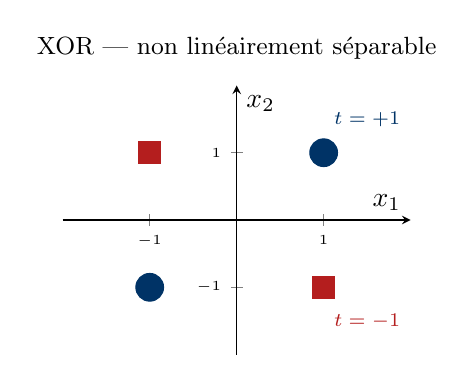
\begin{tikzpicture}
        \begin{axis}[
          width=6.0cm, height=5.0cm,
          xlabel={$x_1$}, ylabel={$x_2$},
          axis lines=center,
          tick label style={font=\tiny},
          xmin=-2, xmax=2, ymin=-2, ymax=2,
          xtick={-1,1}, ytick={-1,1},
          title={\small XOR --- non linéairement séparable},
          title style={font=\small},
        ]
          \addplot[only marks, mark=*, mark size=5pt, jedy_blue]
            coordinates {(-1,-1)(1,1)};
          \addplot[only marks, mark=square*, mark size=4pt, jedy_alert]
            coordinates {(-1,1)(1,-1)};
          \node[jedy_blue,  font=\scriptsize] at (axis cs: 1.5, 1.5) {$t=+1$};
          \node[jedy_alert, font=\scriptsize] at (axis cs: 1.5,-1.5) {$t=-1$};
        \end{axis}
      \end{tikzpicture}
    \end{column}
  \end{columns}
\end{frame}

% ---

\begin{frame}{Vers le Multi-Layer Perceptron (MLP)}
  \begin{columns}[T]
    \begin{column}{0.42\textwidth}
      \textbf{Solution :} empiler des couches avec des
      activations \textbf{non-linéaires}.

      \smallskip
      \begin{block}{Architecture MLP ($L$ couches)}
        \small
        \[
          \bm{h}^{(1)} = \operatorname{ReLU}(\W^{(1)}\bm{x} + \bm{b}^{(1)})
        \]
        \[
          \bm{h}^{(\ell)} = \operatorname{ReLU}(\W^{(\ell)}\bm{h}^{(\ell-1)}
          + \bm{b}^{(\ell)})
        \]
        \[
          \hat{\bm{y}} =
          \operatorname{softmax}(\W^{(L)}\bm{h}^{(L-1)} + \bm{b}^{(L)})
        \]
      \end{block}

      \smallskip
      Le réseau apprend des frontières de décision
      \textbf{courbes et complexes}.

      \smallskip
      \begin{exampleblock}{J3 --- Autograd \& PyTorch}
        \small Comment différencier automatiquement
        toutes ces couches ?\\
        $\Rightarrow$ \textbf{Rétropropagation} \& Autograd.
      \end{exampleblock}
    \end{column}
    \begin{column}{0.54\textwidth}
      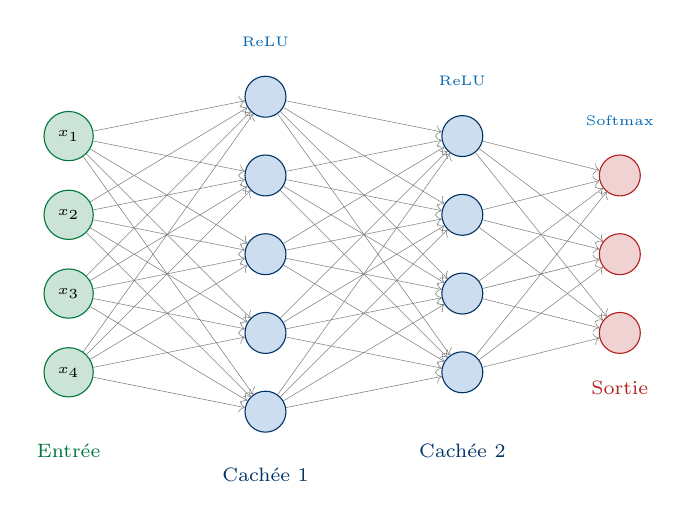
\begin{tikzpicture}[
        nod/.style={circle, draw=jedy_blue, fill=jedy_light,
                    minimum size=0.52cm, font=\tiny},
        inp/.style={circle, draw=jedy_example, fill=jedy_example!20,
                    minimum size=0.52cm, font=\tiny},
        outp/.style={circle, draw=jedy_alert, fill=jedy_alert!20,
                     minimum size=0.52cm, font=\tiny},
        arr/.style={->, gray, very thin},
      ]
        \foreach \i/\y in {1/3.0, 2/2.0, 3/1.0, 4/0.0}
          \node[inp] (i\i) at (0, \y) {$x_\i$};

        \foreach \i/\y in {1/3.5, 2/2.5, 3/1.5, 4/0.5, 5/-0.5}
          \node[nod] (h1\i) at (2.5, \y) {};

        \foreach \i/\y in {1/3.0, 2/2.0, 3/1.0, 4/0.0}
          \node[nod] (h2\i) at (5.0, \y) {};

        \foreach \i/\y in {1/2.5, 2/1.5, 3/0.5}
          \node[outp] (o\i) at (7.0, \y) {};

        \foreach \s in {1,...,4} {
          \foreach \t in {1,...,5} {
            \draw[arr] (i\s) -- (h1\t);
          }
        }
        \foreach \s in {1,...,5} {
          \foreach \t in {1,...,4} {
            \draw[arr] (h1\s) -- (h2\t);
          }
        }
        \foreach \s in {1,...,4} {
          \foreach \t in {1,...,3} {
            \draw[arr] (h2\s) -- (o\t);
          }
        }

        \node[font=\scriptsize, jedy_example] at (0,   -1.0) {Entrée};
        \node[font=\scriptsize, jedy_blue]    at (2.5, -1.3) {Cachée 1};
        \node[font=\scriptsize, jedy_blue]    at (5.0, -1.0) {Cachée 2};
        \node[font=\scriptsize, jedy_alert]   at (7.0, -0.2) {Sortie};

        \node[font=\tiny, jedy_mid] at (2.5, 4.2) {ReLU};
        \node[font=\tiny, jedy_mid] at (5.0, 3.7) {ReLU};
        \node[font=\tiny, jedy_mid] at (7.0, 3.2) {Softmax};
      \end{tikzpicture}
    \end{column}
  \end{columns}
\end{frame}

% ============================================================
% RÉCAPITULATIF
% ============================================================

\begin{frame}{Récapitulatif --- Ce qu'on a vu}
  \begin{columns}[T]
    \begin{column}{0.48\textwidth}
      \begin{block}{Classification Binaire}
        \small
        \begin{itemize}
          \item Labels $t_n \in \{+1,-1\}$,
                hyperplan $\w\T\bm{x}+b=0$
          \item Readout $\operatorname{sign}(f)$ : \textbf{hors} de la loss
          \item $\nabla \operatorname{sign} = 0$
                $\Rightarrow$ GD bloqué
        \end{itemize}
      \end{block}

      \smallskip
      \begin{block}{ReLU \& Perceptron de Rosenblatt}
        \small
        \begin{itemize}
          \item $\operatorname{ReLU}(z) = \max(0,z)$ : dérivée 0/1
          \item $\Loss = \frac{1}{N}\sum \operatorname{ReLU}(-f\cdot t)$
          \item Update : $\w \leftarrow \w + \lr t_n \bm{x}_n$
                si mal classifié
          \item Converge $\Leftrightarrow$ données lin.\ séparables
        \end{itemize}
      \end{block}
    \end{column}
    \begin{column}{0.48\textwidth}
      \begin{block}{Régression Logistique}
        \small
        \begin{itemize}
          \item $\sigma(z) = 1/(1+e^{-z})$ : lisse, $\in (0,1)$
          \item $f_\Theta(\bm{x}) = \sigma(\w\T\bm{x})
                \approx P(t=1|\bm{x})$
          \item Loss : Binary Cross-Entropy,
                encodage $t \in \{0,1\}$
        \end{itemize}
      \end{block}

      \smallskip
      \begin{block}{Multi-Classes \& Vers le MLP}
        \small
        \begin{itemize}
          \item $K$ sorties, encodage one-hot
          \item Softmax $\to$ distribution de probabilité
          \item CCE : $\nabla_{f_k} = p_k - t_k$
          \item Couches cachées + activations $\to$ \textbf{MLP} (J3)
        \end{itemize}
      \end{block}
    \end{column}
  \end{columns}
\end{frame}

% ============================================================
\end{document}
